\documentclass[conference]{IEEEtran}
\IEEEoverridecommandlockouts

\usepackage{iftex}
% Times, as IEEE requires: TeX Gyre Termes under XeTeX (e.g. Tectonic), the standard
% Times setup under pdfLaTeX (e.g. Overleaf). Either way the text is Times.
\ifXeTeX
  \usepackage{fontspec}
  \setmainfont{texgyretermes}[
    Extension = .otf,
    UprightFont = *-regular, BoldFont = *-bold,
    ItalicFont = *-italic, BoldItalicFont = *-bolditalic]
\else
  \usepackage[T1]{fontenc}
  \usepackage{newtxtext}
\fi
\usepackage{cite}
\usepackage{amsmath,amssymb}
\usepackage{graphicx}
\usepackage{booktabs}
\usepackage{url}
\usepackage[hyphens]{xurl}
\usepackage{textcomp}
\usepackage{xcolor}

\graphicspath{{../docs/figures/}}

\begin{document}

\title{Corridor-Level Localisation and Correction of Systematic Route-Planner Error in Road-Freight Logistics}

% One block per author, side by side. The department and institution names are split over two lines so
% that three blocks fit across the page; on one line it pushes the third block down.
\author{
\IEEEauthorblockN{Kuchuru Sai Krishna Reddy}
\IEEEauthorblockA{\textit{Dept. of Computer Science} \\
\textit{and Data Science} \\
\textit{SVKM's Narsee Monjee Institute} \\
\textit{of Management Studies} \\
Hyderabad, India \\
kuchurusaikrishnareddy@gmail.com}
\and
\IEEEauthorblockN{Makkena Lahari}
\IEEEauthorblockA{\textit{Dept. of Computer Science} \\
\textit{and Data Science} \\
\textit{SVKM's Narsee Monjee Institute} \\
\textit{of Management Studies} \\
Hyderabad, India \\
laharisuresh6666@gmail.com}
\and
\IEEEauthorblockN{Shery Mounika Reddy}
\IEEEauthorblockA{\textit{Dept. of Computer Science} \\
\textit{and Data Science} \\
\textit{SVKM's Narsee Monjee Institute} \\
\textit{of Management Studies} \\
Hyderabad, India \\
sherymounikareddy.2006@gmail.com}
}

\maketitle

\begin{abstract}
Production routing engines estimate how long a road-freight leg should take, and on the network studied here they err in one direction almost every time: 98.3\% of 26,369 origin--destination legs run over plan, and the median leg takes $2.0\times$ its planned time. An error that is one-sided is systematic, and a systematic error should be localisable. We test every corridor with at least ten legs against the rest of the network with Welch's $t$-test on log time ratios under Benjamini--Hochberg control at 5\%, and find 273 corridors significantly slower and 512 significantly faster than the network, together covering 78.6\% of legs. The answer depends heavily on one parameter: raising the support floor from ten legs to thirty yields a top-20 list with no corridor in common. For prediction, a gradient-boosted model trained on the residual over a per-corridor median reaches 30.90 minutes mean absolute error against the median's 33.04, winning on all fourteen evaluation slices, with most of the gain on corridors without history. A streaming pipeline serves the model from event-time state and reproduces the batch predictions exactly on every leg. We also report two evaluation traps: an optimiser default that silently disabled the loss the model was chosen for, and a replay that scored early events against later history and inflated an alert precision from 58.6\% to 72.1\%.
\end{abstract}

\begin{IEEEkeywords}
logistics, route planning, travel-time reliability, multiple testing, gradient boosting, stream processing, language-model agents
\end{IEEEkeywords}

% ─────────────────────────────────────────────────────────────────────────────
\section{Introduction}

A route planner's estimate is a plan, and a plan that is consistently optimistic remains useful if the operator knows \emph{where} it is optimistic. The public trip records of Delhivery, an Indian road-freight carrier~\cite{delhivery}, carry both the production engine's planned time and the realised time for every leg, which makes that question answerable directly from operational data rather than by simulation.

The starting observation is simple (Fig.~\ref{fig:premise}). Across 26,369 legs, 98.3\% exceed their planned time and the median leg runs at twice its plan. If the error were noise it would centre on one and cancel within a corridor. It neither centres nor cancels, so it should concentrate somewhere. We make four claims, in order of importance:
\begin{enumerate}
\item \textbf{An FDR-controlled corridor audit localises the planner's error}: of 1,130 corridors tested, 273 are significantly slower and 512 significantly faster than the network (Section~\ref{sec:audit}).
\item \textbf{The support threshold decides the answer}: at floors of 10 and 30 legs the top-20 lists are disjoint, a methodological warning for any corridor-level ranking (Section~\ref{sec:support}).
\item \textbf{A residual correction over the fair baseline} reaches 30.90 minutes against a per-corridor median's 33.04 and wins on every slice, with the gain concentrated where the baseline has no history (Section~\ref{sec:model}).
\item \textbf{Two evaluation traps we fell into and report}: an optimiser setting that made the chosen loss inert, and a streaming replay that leaked future history into alert scoring (Sections~\ref{sec:optimiser} and~\ref{sec:replay}).
\end{enumerate}

We also describe the surrounding system---a streaming path that serves the reported model with predictions identical to batch, and a small agent layer built on a deliberate design position---because the evaluation findings only make sense in that context. We do not claim to beat the production planner: OSRM has no access to corridor history, and a model that does is not a fair comparison. OSRM is reported as context throughout.

\begin{figure}[t]
\centering
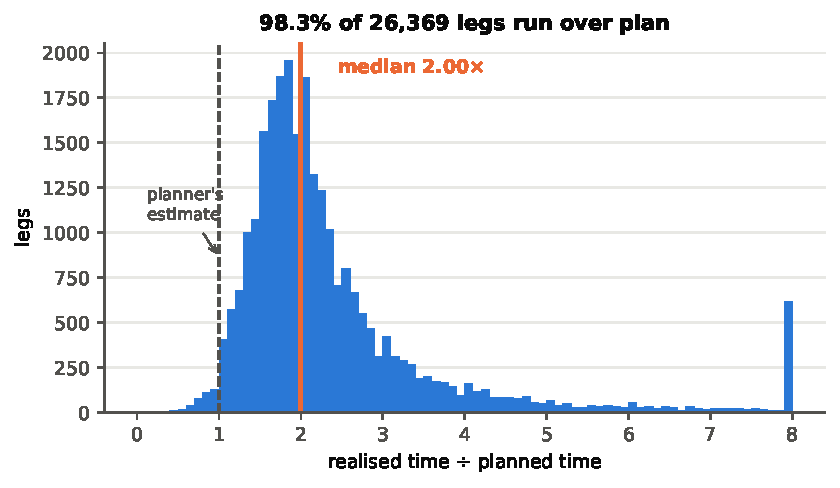
\includegraphics[width=0.88\columnwidth]{fig1_gap_ratio_distribution.pdf}
\caption{Distribution of realised over planned time across 26,369 legs. The mass sits well to the right of 1.0: 98.3\% of legs run over plan and the median ratio is 2.0.}
\label{fig:premise}
\end{figure}

% ─────────────────────────────────────────────────────────────────────────────
\section{Related Work}

\textit{Route engines as the thing measured.} The planned times in our data come from OSRM, an open-source route planner over OpenStreetMap data~\cite{osrm}. A route engine estimates the travel time of the best route from per-road-class speed profiles; it has no notion of hub dwell, loading or a particular corridor's history. Our audit treats its estimate as a measurement to be checked against outcomes, corridor by corridor.

\textit{Residual prediction over a route engine.} DeeprETA~\cite{deepreta} post-processes a route planner's ETA with a deep residual network and reports lower mean and median absolute error than competitive regression baselines at very high query volume. Our formulation was arrived at independently and has the same structure---predict the correction, not the total. We differ in aim, treating the model as secondary to localising where the engine is wrong; in scale; and in reporting the correction's behaviour by slice.

\textit{Delivery-time prediction.} Gradient boosting is a strong and inexpensive baseline for delivery times; on postal data, LightGBM and CatBoost were the most accurate and efficient of the models compared~\cite{khiari2020}. Wen \textit{et al.}~\cite{wen2023survey} survey route and time prediction for instant delivery; by their taxonomy this work is time-only, supervised and non-deep, on line-haul freight measured in hours rather than urban delivery measured in minutes. Deep models for pick-up route prediction~\cite{drl4route} and for timely-rate prediction under anomalies~\cite{deepsta} address adjacent problems with far richer trajectory data.

\textit{Corridor-level travel-time reliability.} Transport research characterises freight corridors with descriptive reliability indices---planning-time and buffer indices, percentile spreads, fitted distributions---usually from GPS probe data~\cite{fhwa}. We share the unit of analysis and add significance testing with multiplicity control~\cite{welch1947,bh1995}, which turns ``this corridor looks unreliable'' into ``this corridor is slower than the network at a 5\% false discovery rate''.

\textit{Language-model agents for operations.} Agents that interleave reasoning with tool calls~\cite{react} are now surveyed as a field~\cite{wang2024survey}, and the Model Context Protocol~\cite{mcp} standardises how such agents reach tools and data. Closest to our design position is OptiGuide~\cite{optiguide}, in which a language model answers supply-chain questions by editing an optimiser's input and explaining its output while the optimiser makes the decision. Our agents apply the same division more strictly: every verdict is computed by code, and the model writes only the sentence a person reads.

\textit{Control towers.} In supply-chain practice a control tower is a central point of visibility and coordination over shipments; Trzuskawska-Grzesi\'{n}ska collects business cases and argues that whole-chain visibility requires control towers to be integrated with one another~\cite{controltower}. Our system takes the name for the same role and contributes an evaluated prototype.

\textit{On this dataset.} Searches in September and October 2026 found feature-engineering notebooks and case studies using the Delhivery records, typically comparing actual and OSRM time, but no peer-reviewed study. With no published result to place in a comparison row, every result below is reported beside a trivial policy computed on the same data.

% ─────────────────────────────────────────────────────────────────────────────
\section{Data and Preparation}

The raw records are 144,867 scan-level segments across 14,817 trips collected between 12 September and 8 October 2018. Cleaning repairs types and keys and flags 2,600 suspect segments without dropping any row. Segments are reconstructed into 26,369 origin--destination \emph{legs} on 2,783 \emph{corridors}, where a corridor is an ordered pair of facilities; the legs touch 1,657 facilities. A leg is one trip's movement from one facility to the next, keyed by trip, corridor and departure time, because a trip can repeat a corridor on another day.

\textit{Dwell is separated from movement.} The realised moving time excludes dwell at the hub, which is the scan-to-scan interval minus moving time. The median leg spends 49 minutes, 34.6\% of its wall clock, parked. The distinction matters twice. A leg finishes at its final scan, not at departure plus moving time: an earlier version of our pipeline used the latter, placed every finish a median 49.6 minutes early and counted unfinished legs as history. And a leg is called delayed when it exceeds $2.0\times$ its plan; at that threshold 49.65\% of legs are delayed, against 93.62\% at the $1.25\times$ threshold first considered.

\subsection{As-of Features}
Every feature describing a corridor's or a hub's history is computed only from legs that had \emph{finished} before the leg being predicted was \emph{created}, with completions ordered before creations on a tie. Under this rule 11.09\% of legs have no prior history on their corridor; they carry an explicit cold-start indicator rather than a zero that would read as ``known to be on time''. Because a leakage rule is a claim, we verified it: an independent reconstruction of the as-of history agrees with the production implementation on 100\% of legs with history. Before the finish-time correction above the agreement was 95.2\%, which is how that error was found.

% ─────────────────────────────────────────────────────────────────────────────
\section{The Corridor Audit}\label{sec:audit}

\subsection{Method}
For each leg the statistic is the logarithm of realised over planned time, which makes the comparison multiplicative and symmetric. Each corridor with at least ten legs is tested against the rest of the network with Welch's unequal-variance $t$-test~\cite{welch1947}. The comparison group's sums are obtained by subtracting the corridor's own from the network totals, so all 1,130 tests need a single pass over the data. The $p$-values are corrected by the Benjamini--Hochberg procedure at 5\%~\cite{bh1995}.

\subsection{Result}
Of the 1,130 corridors tested, \textbf{273 are significantly slower and 512 significantly faster} than the network, and the tested corridors cover 20,739 of 26,369 legs (78.6\%) (Fig.~\ref{fig:audit}). The worst corridor runs at $13.9\times$ the network's typical overrun, and 70 of the 273 slow corridors are intra-city, an operational problem distinct from long-haul delay. That more corridors are confirmed faster than slower is itself informative: the planner's optimism is not uniform, and a single network-wide correction factor would make 512 corridors worse.

\begin{figure}[t]
\centering
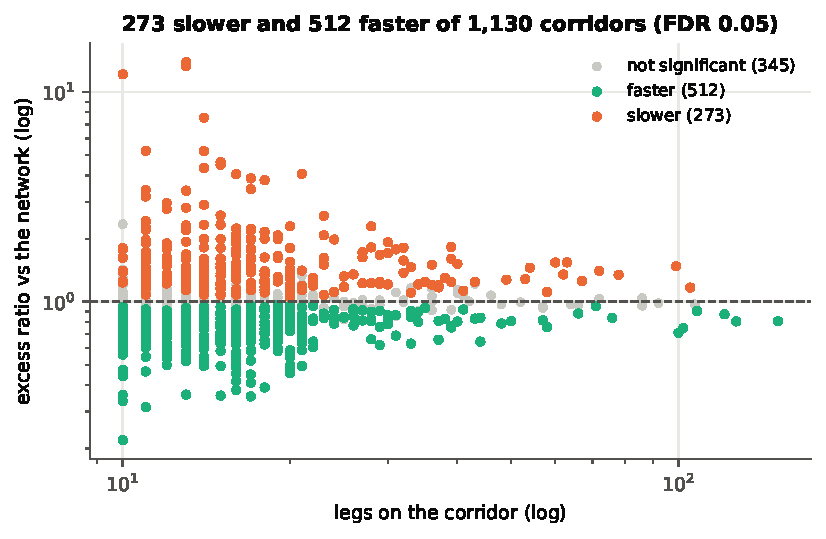
\includegraphics[width=\columnwidth]{fig2_corridor_audit.pdf}
\caption{The corridor audit: 1,130 corridors tested against the rest of the network; 273 significantly slower and 512 significantly faster at a 5\% false discovery rate.}
\label{fig:audit}
\end{figure}

\subsection{The Support Threshold Decides the Answer}\label{sec:support}
At a 30-leg floor only 99 corridors are testable; 34 are significantly slower and 36 faster, and the worst runs at $1.92\times$. Its top-20 list shares \textbf{no corridor} with the 10-leg list, and its worst corridor is milder than the 10-leg list's fifteenth (Fig.~\ref{fig:support}). Neither list is wrong. A higher floor keeps only heavily used corridors, which are systematically less extreme; a lower floor admits thinly observed corridors whose large effects survive false-discovery control because they are large. A ranking of bottlenecks is therefore conditional on a support choice that analyses rarely state. We state ours and argue that any corridor-level ranking should be reported at two floors at least.

\begin{figure}[t]
\centering
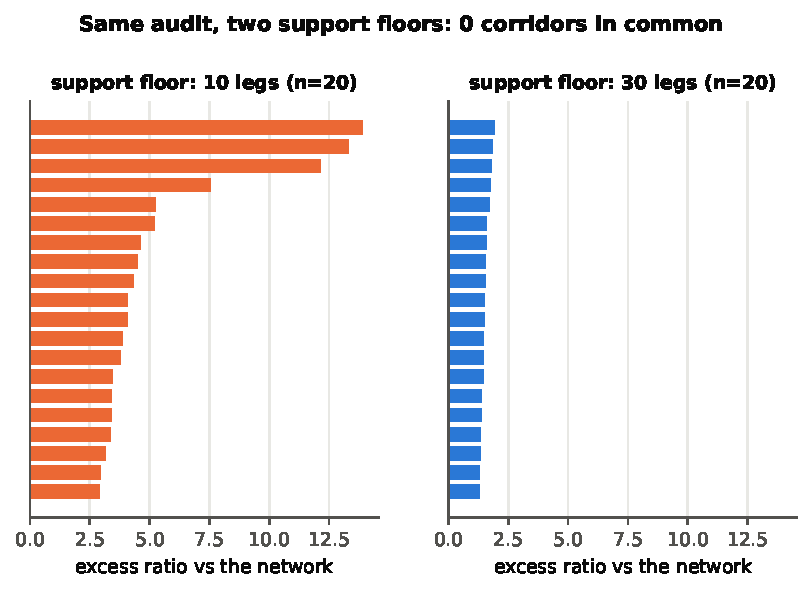
\includegraphics[width=\columnwidth]{fig4_support_instability.pdf}
\caption{Top-20 slow corridors at support floors of 10 and 30 legs. The two lists share no corridor.}
\label{fig:support}
\end{figure}

% ─────────────────────────────────────────────────────────────────────────────
\section{Predicting the Gap}\label{sec:model}

\subsection{Setup and Baselines}
The quantity predicted is the \emph{gap}: how many minutes past its plan a leg will run, known at the moment the leg is created. The split is chronological---21,095 legs for training and the latest 5,274 for test---because a random split scores a model on legs interleaved in time with its training data. The metric is mean absolute error (MAE) in minutes, and the fair baseline follows from it: MAE is minimised by the median, so the right comparator is the per-corridor as-of \emph{median}, not the mean (Table~\ref{tab:mae}). Using the mean as the bar would have flattered every model by 3.1 minutes.

\begin{table}[t]
\caption{Test MAE on 5,274 legs}
\label{tab:mae}
\centering
\begin{tabular}{@{}lr@{}}
\toprule
Model & MAE (min) \\
\midrule
OSRM plan (context) & 107.09 \\
Random forest, squared loss, raw target & 36.89 \\
Per-corridor mean & 36.13 \\
\textbf{Per-corridor median (the bar)} & \textbf{33.04} \\
GBT on median residual, step size 0.05 & 32.52 \\
\textbf{GBT on median residual, step size 1.0} & \textbf{30.90} \\
Single-node reference, absolute loss & 29.52 \\
\bottomrule
\end{tabular}
\end{table}

\subsection{Residual Formulation}
The model is trained on the gap minus the corridor median, and its prediction is added back to the median, so a model that learns nothing reproduces the baseline exactly. Its 38 inputs are the leg's planned time and distance, departure hour, day and route type; as-of history for the corridor and both hubs with cold-start flags; and a second table adding corridor dispersion (median, 90th percentile, interquartile range, standard deviation), a trailing seven-day corridor mean, and hub dwell by part of the day. The learner is a gradient-boosted tree ensemble of 200 trees of depth 6 with absolute loss, because MAE is the reported metric.

\subsection{Selection Protocol}
The one hyperparameter varied, the step size, was chosen on a second chronological cut inside the training split; the chosen model was refit on the full training split and scored once on test. We fixed this procedure in writing before running it, including the commitment to adopt whatever the test score turned out to be. On validation every step size lost to the median, the best by 30.17 against 29.89; on test the chosen one won by 6.5\%. We applied the rule as written and report both results, because the second qualifies the first.

\subsection{An Optimiser Setting that Disabled the Loss}\label{sec:optimiser}
Our first residual model, absolute-loss boosting at a step size of 0.05, reached 32.52---clearing the bar by 1.6\%, yet losing to the median on every corridor with history; its whole margin came from 294 legs on unseen corridors. Reading the saved model explained why. The library's absolute-loss boosting fits its first tree to the raw target with squared error, with leaf values from $-1{,}382$ to $+2{,}605$ minutes, and every later tree to the \emph{sign} of the error, with leaf values in $[-1, 1]$ scaled by the step size. At 0.05, the 199 corrective trees can move a prediction by at most 9.95 minutes in total: the loss the model was chosen for was barely switched on. Validation over step sizes $\{0.05, 0.3, 1.0\}$, with correction caps of 9.95, 59.7 and 199 minutes, confirmed the mechanism in the ordering of the results.

\subsection{Where the Gain Is}
The reported model wins on all fourteen slices by corridor support, route type, distance band and departure hour. Most of the margin, however, comes from the 294 test legs whose corridor had no history in training, where the error falls from 111.2 to 75.9 minutes; on corridors with history the model beats the median by 0.02 to 0.51 minutes (Fig.~\ref{fig:support_mae}). The model is a large improvement where a lookup table has nothing to say, and a small one everywhere else. The single-node reference's 29.52 marks the headroom that remains for the distributed configuration.

\begin{figure}[t]
\centering
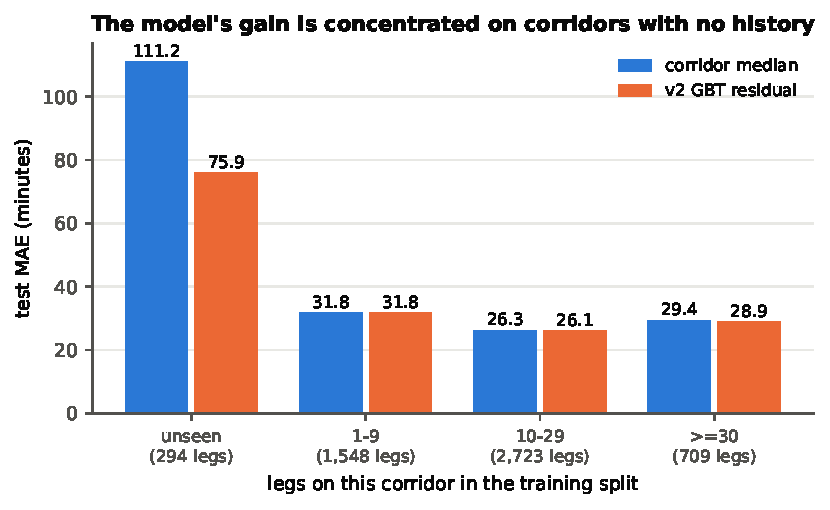
\includegraphics[width=\columnwidth]{fig6_mae_by_support.pdf}
\caption{MAE by corridor support in training. The gain over the median is concentrated on corridors unseen in training.}
\label{fig:support_mae}
\end{figure}

% ─────────────────────────────────────────────────────────────────────────────
\section{Streaming and Serving}

A producer replays legs as two kinds of event---a \emph{query} when a leg is created and a \emph{fact} when it finishes---and a structured-streaming job scores each query and raises an alert when the prediction crosses twice the planned time. Several features cannot be served from a static lookup: a seven-day window moves with each query, and dwell is keyed by hub and by the query's own part of the day. The job therefore keeps every corridor's and hub's history as \textbf{event-time state}: each fact updates the state of the keys it belongs to, each query reads that state as of its own time, and the state is persisted so that a restarted job resumes with the history it had. The state updates repeat the batch arithmetic in the same order, so results are equal rather than close.

\textit{Equivalence.} Over the full 52,738-event replay, run in two halves across a restart from the persisted state, \textbf{all 26,369 legs score bit-identically to batch}, no history feature differs on any leg, and the stream's own test-split predictions give the reported 30.90 minutes. Replaying the same 2,000 legs through a live message broker and through a file source produces the same 1,347 alerts on the same legs with the same predicted gaps.

\textit{Throughput.} With a stateless history lookup, the producer sustained 886 events/s and the job scored 740 events/s, with event-to-alert latency of 28.9\,s at the median and 38.0\,s at the 95th percentile on one 20-core machine. Event-time state costs throughput: the stateful job scored 74 events/s of busy time on the same machine, ample for the real event rate and too slow for a one-minute replay of three weeks. A public interface serves the same model with a tree evaluator identical to the distributed one on every leg, at 345\,ms at the 95th percentile.

\textit{Alerting is a workload decision.} For the best classifier, raising the delay threshold from $1.15\times$ to $2.0\times$ moves the Matthews correlation only from 0.507 to 0.536, while the share of legs alerted falls from 98\% to 49\% (Fig.~\ref{fig:threshold}). The threshold is a policy about how many alerts an operator can act on, not a dial for quality.

\begin{figure}[t]
\centering
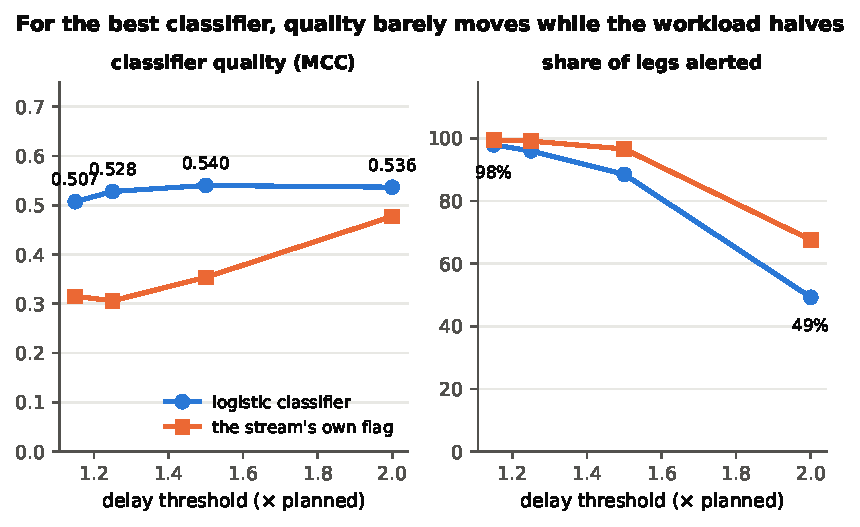
\includegraphics[width=0.88\columnwidth]{fig7_threshold_sensitivity.pdf}
\caption{Matthews correlation and alert volume across delay thresholds. Quality is nearly flat; workload is not.}
\label{fig:threshold}
\end{figure}

% ─────────────────────────────────────────────────────────────────────────────
\section{The Agent Layer as a Design Position}

\subsection{Verdicts Computed, Prose Generated}
Five agents---document extraction, order entry, exception triage, invoice audit and an analytics assistant---share one rule: every verdict is computed, and a language model writes only the sentence a person reads. Severity is arithmetic over how far past its threshold a leg is predicted to run; an invoice verdict is four comparisons. The rule makes each decision reproducible and therefore scorable, and bounds what a model error can do to a sentence. Each agent's evaluation set was authored by someone other than its builder, and every result is reported beside a trivial policy on the same set.

On small first sets, order entry filed or clarified 50 of 50 templated emails correctly with no invented order; invoice audit disputed with 100\% precision and 82.2\% recall; document extraction scored 97.9\% of fields on 20 of 40 planned rows; and the assistant's model-written answers were grounded in 17 of 18 cases, with all six out-of-scope questions refused. A perfect score on twenty cases is consistent with a true rate of 84\%, so the agents were re-run at scale, stratified so that hard cases form a named share, with Wilson 95\% intervals. Order entry scored \textbf{85.0\% [79.4, 89.3] on 200 held-out emails}, falling to 70.0\% on the adversarial half, where every error was an order filed on a value the email never stated. Invoice audit was correct on \textbf{90.0\% [85.1, 93.4] of 200 invoices} with no correct invoice disputed; its misses are the one kind that falls inside its own tolerance. The orchestrator routed \textbf{100 of 100} lifecycles as the email deserved, exercising all three paths through its graph.

The one groundedness failure is instructive. Asked how many corridors are statistically slower, the model counted the three slow corridors among its five retrieved passages and answered ``3''. Every number was in its context, so a mechanical check passed it; the error was the generalisation. Conversely, asked which hub has the longest dwell \emph{time}, the model answered from the numbers it was given and was right where our own ranking, sorted by dwell \emph{share}, was wrong.

\subsection{A Replay that Scored the Past with the Future}\label{sec:replay}
The exception agent's notification precision was first measured at 72.1\% against 54.1\% for alerting on every leg. The measurement replayed the earliest 2,000 legs through a version of the streaming job that joined each query to the latest history snapshot. Live, that is history up to now; in a replay it is history up to the end of the data. 1,290 of the 2,000 replayed legs had no corridor history at their own creation time and were scored as if they had fourteen prior legs. Scoring the same legs with only the history each had at its own time gives a precision of \textbf{58.6\%}, and by severity 39.7, 51.3, 76.6 and 85.3\% against 53.2, 68.6, 85.1 and 91.8\% as first measured (Fig.~\ref{fig:severity}). The snapshot run reproduces the first measurement exactly, so the gap is the leak and nothing else. Precision still rises with severity, so the grade is a useful filter, but the gain over the trivial policy is 4.5 points, not 18. A replay is an evaluation only if every join inside it is as-of the event being replayed.

\begin{figure}[t]
\centering
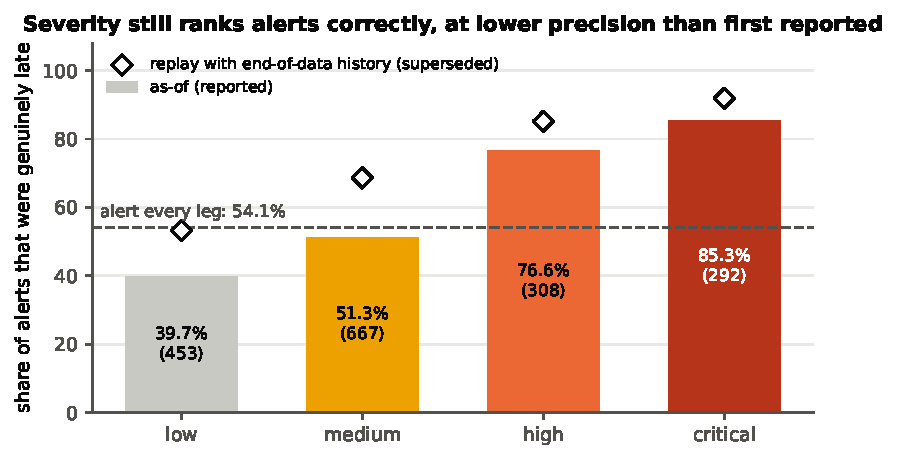
\includegraphics[width=\columnwidth]{fig9_severity_precision.pdf}
\caption{Notification precision by severity, as first measured with end-of-data history and as measured with as-of history.}
\label{fig:severity}
\end{figure}

\subsection{What the Language Model Adds: An Ablation}
The design position makes a direct question answerable: what does each agent lose or gain when the language model is removed, or given the decision? Table~\ref{tab:ablation} places the measured configurations side by side; a dash marks a configuration not measured, not an assumed result.

\begin{table*}[t]
\caption{Agent configurations. \textit{Rules}: code decides and templates write. \textit{+ LLM phrasing}: the same decision, worded by the model. \textit{LLM decides}: the model makes the decision. \textit{Human}: a second person's labels.}
\label{tab:ablation}
\centering
\begin{tabular}{@{}lllll@{}}
\toprule
Agent (set) & Rules & Rules + LLM phrasing & LLM decides & Human \\
\midrule
Order entry (50 emails) & 50/50 & --- & 50/50 & --- \\
Order entry (200 emails, held out) & 85.0\% [79.4, 89.3] & --- & --- & --- \\
Assistant: route accuracy (30 questions) & 90.0\% & 93.3\% & --- & --- \\
Assistant: out-of-scope refused & 3/6 & 4/6 model layer; 6/6 both layers & --- & --- \\
Assistant: answers grounded & extractive & 17/18 & --- & --- \\
Exception agent: precision (as-of) & 58.6\% & same verdicts & --- & --- \\
Document extraction (20 rows) & --- & --- & 97.9\% of fields & --- \\
\bottomrule
\end{tabular}
\end{table*}

On the 50-email set the model deciding and the rules deciding are indistinguishable, so that set cannot separate them; separating them needs the 200-email set scored with the model deciding, which a free-tier budget of 20 model calls a day has not yet allowed. Where the model only phrases, its measurable contribution is at the edges: three more points of route accuracy and one more refusal, at the cost of one ungrounded answer in eighteen. Document extraction is the one agent where the model decides and no rule baseline exists, and it rests on 20 of 40 planned rows. The empty human column is the clearest gap: no agent decision has yet been compared against a second labeller.

% ─────────────────────────────────────────────────────────────────────────────
\section{Scale}

The audit's two aggregation functions, imported unchanged, were run on New York City taxi trip records mapped into the leg shape; the planned time there is a stated stand-in, and no gap statistic is reported from those data. \textbf{56,353,613 rows aggregate in 14.32\,s on 20 cores}, 3.9 million rows per second (Fig.~\ref{fig:scale}). Two readings are unflattering and belong here: at this project's own size the runtime is the engine's fixed cost---26,369 legs and 2.9 million trips both take 2.4\,s---and five times the cores bought only $1.24\times$ the speed, because reading 914\,MB from one disk is IO-bound.

\begin{figure}[t]
\centering
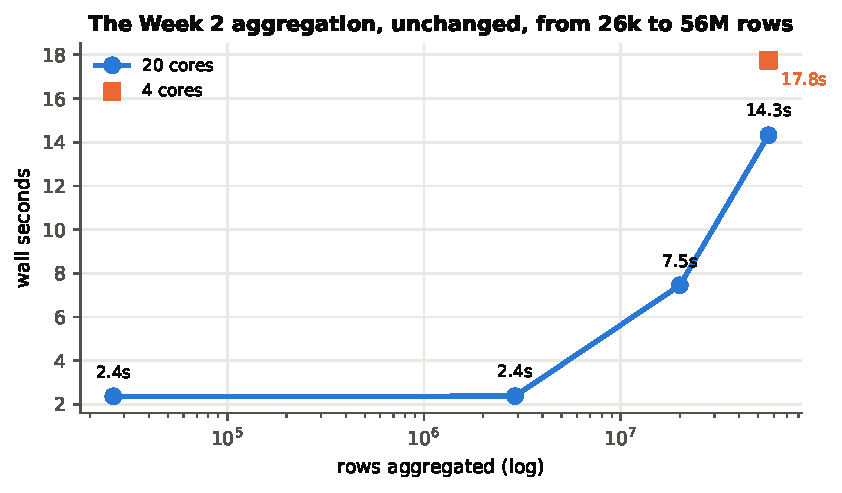
\includegraphics[width=0.88\columnwidth]{fig8_scale_runtime.pdf}
\caption{Aggregation runtime against input size and core count.}
\label{fig:scale}
\end{figure}

% ─────────────────────────────────────────────────────────────────────────────
\section{Threats to Validity}

\textit{External validity.} Every network result describes one operator's network in one country over 22 days of leg creation, from 12 September to 3 October 2018. Whether the corridors the audit flags are stable over months or across carriers is untested, and the window is too short to show seasonal drift. The data record that a leg ran late, not why.

\textit{Construct validity.} The agents read documents, emails and invoices generated for this study and post to a mock transport management system. Their scores measure the pipeline against our own generator rather than the world; the invoice auditor's rate band is the corpus's own pricing model and says nothing about real freight rates. Only the network data are real.

\textit{Internal validity.} A streaming replay joined every query to end-of-data history and inflated a precision from 58.6\% to 72.1\% (Section~\ref{sec:replay}). The served model now uses event-time state, which is as-of by construction, and the measurement that matters was re-run as-of; any further replay-based measurement inherits the risk, and a stream-equals-batch test on feature rows alone would not catch it.

\textit{Statistical conclusion validity.} Agent evaluations range from 20 to 200 cases; small sets are reported with their size and the 200-case runs with Wilson intervals. Document extraction rests on 20 of 40 planned rows, the assistant's groundedness on 18 judged answers. For the model, the validation cut favoured the median baseline while the test split favoured the model; both are reported, and adoption followed a rule fixed before the test split was scored.

\textit{Evaluator independence.} Each agent's set was authored by someone other than its builder, but no decision has been labelled by a second person to measure agreement, and the groundedness judgements were made by one reader.

% ─────────────────────────────────────────────────────────────────────────────
\section{Conclusion}

A production planner's error on this network is systematic and localisable: an FDR-controlled audit identifies the corridors where it is wrong in either direction, and the choice of support floor changes which ones. A residual model over a per-corridor median improves prediction most where history is absent, and is served from event-time state with predictions identical to batch on every leg. Two of our findings concern evaluation rather than the network---an optimiser default that disabled the chosen loss, and a replay that leaked the future into alert scoring---and both were found only by comparing a number with the same number computed another way. Future work: scoring the agents with the model deciding at scale and against a second labeller, a live-deployment evaluation of alert precision, and extending the audit to a longer period to test whether the corridors it flags are stable.

\section*{Data and Code Availability}
The source data are public~\cite{delhivery} and are not redistributed. All code, the decision log, every result file behind the numbers above, a model card and a data card are available at \url{https://github.com/krishna-2-005/Agentic-AI-Logistics-Control-Tower}; an interactive version of the results is at \url{https://control-tower-mu-rouge.vercel.app}.

\section*{Acknowledgment}
During the preparation of this work the authors used a generative AI assistant to help draft and edit text and code. The authors reviewed and edited all content, verified every number against the underlying result files and every reference against its source, and take full responsibility for the publication. \textcolor{red}{[Adjust to the venue's policy before submission.]}

\bibliographystyle{IEEEtran}
\bibliography{references}

\end{document}
